% Validation pyramid — compact cheat-sheet variant.
% Smaller widths, abbreviated layer labels, dropped cost-per-run column
% (the layer reference table below the figure carries that info).
\documentclass[tikz,border=4mm]{standalone}
\usepackage{tikz}
\usetikzlibrary{positioning, arrows.meta}

\begin{document}
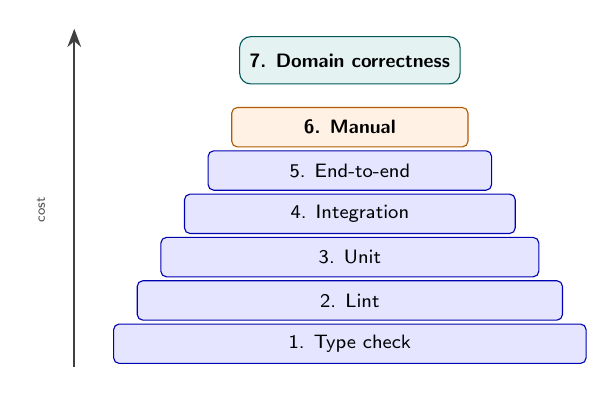
\begin{tikzpicture}[
  font=\sffamily,
  layer/.style={
    draw=blue!70!black, fill=blue!10,
    minimum height=0.5cm, align=center, font=\sffamily\scriptsize,
    rounded corners=2pt
  },
  apex/.style={layer,
    draw=orange!70!black, fill=orange!10,
    font=\sffamily\scriptsize\bfseries
  },
  human/.style={
    draw=teal!70!black, fill=teal!10,
    minimum height=0.6cm, align=center, font=\sffamily\scriptsize\bfseries,
    rounded corners=4pt
  },
]

\node[layer, minimum width=6cm]   (l1) at (0, 0)    {1. Type check};
\node[layer, minimum width=5.4cm] (l2) at (0, 0.55) {2. Lint};
\node[layer, minimum width=4.8cm] (l3) at (0, 1.10) {3. Unit};
\node[layer, minimum width=4.2cm] (l4) at (0, 1.65) {4. Integration};
\node[layer, minimum width=3.6cm] (l5) at (0, 2.20) {5. End-to-end};
\node[apex,  minimum width=3.0cm] (l6) at (0, 2.75) {6. Manual};

% Layer 7 separated above
\node[human, minimum width=2.8cm] (l7) at (0, 3.6) {7. Domain correctness};

% Cost arrow on left (thin, with short label)
\draw[-Stealth, thick, draw=gray!50!black] (-3.5, -0.3) -- (-3.5, 4.0);
\node[font=\sffamily\tiny, text=gray!60!black, rotate=90, anchor=south] at (-3.75, 1.7) {cost};

\end{tikzpicture}
\end{document}
